\documentclass[12pt,journal]{IEEEtran}

\usepackage[pdftex]{graphicx}
\DeclareGraphicsExtensions{.png}

\usepackage{cite}
\usepackage{setspace}
\usepackage{amsmath}
\usepackage{hyperref}


\begin{document}

\title{CSCI 580 : Monte Carlo Path Tracing}
\markboth{Thursday~December~3\textsuperscript{rd}~2015}
{December~3\textsuperscript{rd}~2015}
\author{
	Sincennes, Alexandre
	\texttt{sincenne@usc.edu}\\
	\and
 	Peechankottil Manikandan, Sajini
 	\texttt{smanikan@usc.edu}\\
  	\and
	Guanzhou Liu, Vincent
 	\texttt{guanzhol@usc.edu}\\
  	\and
	Ramirez, Bernie
 	\texttt{berniera@usc.edu}\\
  
}
\maketitle

%===================================================

\section{Abstract}
A Monte Carlo path tracing renderer was created using the assignment application as a base. Realistic images featuring shadows and diffuse interreflections become crisp beyond 20 sets of generated rays, with a recursion depth greater than or equal to 4.

%===================================================

\section{Introduction}
Rendering via the use of rays, such as in the Monte Carlo path tracing approach, stands in stark contrast to the rasterization of triangles, which is the faster and more common approach to rendering, and the one used throughout the assignments of the CSCI 580 course. However, with path tracing it is possible to achieve photorealism by simulating the travel of light, which bounces off surfaces, resulting in shadows, specular as well as diffuse reflections and refractions rather than the surface shading approach used in renderers that make use of rasterization.

%===================================================

\section{Prior Work}
The origins of path tracing begin with ray tracing, first outlined in A. Appel's 1968 paper[1]. In the ray tracing technique, rays are cast out from the camera, or eye, through the image plane, and into the scene. The first surface it collides with is the one rendered for that pixel. Additionally, rays called shadow rays are cast from the light sources and determine whether or not the surface is being occluded by another, which would be collided with first by the shadow ray. A further development was Whitted ray tracing[2], wherein rays generate new rays upon collision with a surface, for direct illumination, perfect refraction and perfect reflection.

\par

Also instrumental for Monte Carlo path tracing was work in radiosity, which takes into account lighting emitted from diffuse surfaces rather than specular reflection. J. Kajiya's 1986's paper[3] on the rendering equation brings a mathematical basis for these relationships, described by:

\begin{center}
$L_{\text{o}}(\mathbf x,\, \omega_{\text{o}},\, \lambda,\, t) \,=\, L_e(\mathbf x,\, \omega_{\text{o}},\, \lambda,\, t) \ +\, \int_\Omega f_r(\mathbf x,\, \omega_{\text{i}},\, \omega_{\text{o}},\, \lambda,\, t)\, L_{\text{i}}(\mathbf x,\, \omega_{\text{i}},\, \lambda,\, t)\, (\omega_{\text{i}}\,\cdot\,\mathbf n)\, \operatorname d \omega_{\text{i}}$
\end{center}

\begin{flushright}
\par 
(1)
\end{flushright}

\par
Monte Carlo path tracing combines the techniques of reflected or refracted rays by recursively generating other rays, but also captures the lighting relations between diffuse surfaces. We implemented it with ray reflections in a random uniform fashion, with a deterministic number of reflected rays or until the ray hits a light source.

\section{The Monte Carlo Path Tracing Algorithm}
The core of the Monte Carlo algorithm is recursive and has relatively few steps. It can be summed as thus(modified version of an algorithm found in [4]):

\begin{description}
  \item[1)] Generate a ray from the camera (position x,y, horizontal and vertical fields of view u,v), passing through the image plane, with $weight = 1$
  \item[2)] Find the point of intersection with the nearest surface
  \item[3)] Determine whether the surface is a light source or not (as indicated by a special coefficients for light emittance)
  \item[3A)] if it is a light source, return $weight * light$
  \item[3B)] if not, $weight \mathrel{*}= \frac{Ks+Kd+Ka}{3}$ and randomly scatter a new ray according to a probability density function (pdf) approximating its bidirectional refletance distribution function (brdf), and go to step 2
\end{description}

\newpage

In order for this algorithm to be implemented, other algorithms such as ray-triangle intersection must also be implemented. 
Additionally, a BRDF pdf must be created for each surface. A reasonable BRDF pdf would be a uniform distribution, wherein \emph{any} 
vector (x,y,z) which is in the hemisphere of the surface is randomly selected.

\section{Application Structure}
Firstly, we used the codebase of the previous assignments as a launching point for the project. Thus, the GUI and initialization, as well other elements such as the rendering parameters, the functions for displaying pixels to the screen and a number of vector and matrix functions were borrowed directly from previous assignments. However, rasterization-related functionality was thrown out and replaced with an entirely new way of rendering via rays.

\section{Graphics Pipeline}
The graphics pipeline was designed as follows: initialization is carried out, wherein global properties such as camera position and lights are defined. Then, the meshes are loaded into memory as a data structure encompassing all triangles. Each vertex in the triangle has a position and a normal in world space coordinates, as well as information on their specular, diffuse and ambient coefficients, which differs from the global Ks, Kd and Ka found in the assignment renderer. Also associated with vertices is a lighting coefficient for surfaces which emit light. Next, this set of all geometry is used by the path tracing technique to determine colour at each pixel, which is finally fed to the same display as the one used in previous asignments.

\section{The Path Tracing Implementation}
Much like the Monte Carlo path tracing algorithm outlined previously, rays are cast from the camera out into the scene, through the view plane. The reason for why the process is carried out in the reverse order in comparison to the real world, in which light is emitted from a light source, bounces off surfaces and hits the film or photoreceptors (or the real-world ``image plane'') of the camera, is that in reality, the vast majority of light misses this ``image plane''. Therefore, it would be extremely inefficient to calculate the path of light beams (or photons) which would be unseen by the camera.
\par
If we know the vertical and horizontal fields of view of the camera, as well as its position (e, for eye) and coordinate system (u,v,n) as well as picking an arbitrary distance (d) for the view plane, we can determine the height ($h$) and width ($w$) of the image plane:

\begin{center}
$\tan(\theta_{vertical}/2) = h / 2d$
\end{center}

\begin{flushright}
\par 
(2)
\end{flushright}

\begin{center}
$\tan(\theta_{horizontal}/2) =w / 2d$
\end{center}

\begin{flushright}
\par 
(3)
\end{flushright}

Then, we can find the center of the image plane, and its bottom-left corner ($BL$):

\begin{center}
$c = e - n * d$
\end{center}

\begin{flushright}
\par 
(4)
\end{flushright}

\begin{center}
$BL = c - u * h /2 - v *w/2$
\end{center}

\begin{flushright}
\par 
(5)
\end{flushright}

Finally, with knowledge of the image resolution ($w_{i}$ and $h_{i}$), we can find the location of the pixel that the ray will pass through:

\begin{center}
$\text{pixel}_{(i,j)}= BL + u * i * w / w_{i} + v * j * h/h_{i}$
\end{center}

\begin{flushright}
\par 
(6)
\end{flushright}

Thus, with the position of the pixel we want to draw on the image plane, and the position of the camera, we can draw a ray starting at the camera, passing through that pixel, and into the environment.

\begin{figure}[!t]

\centering
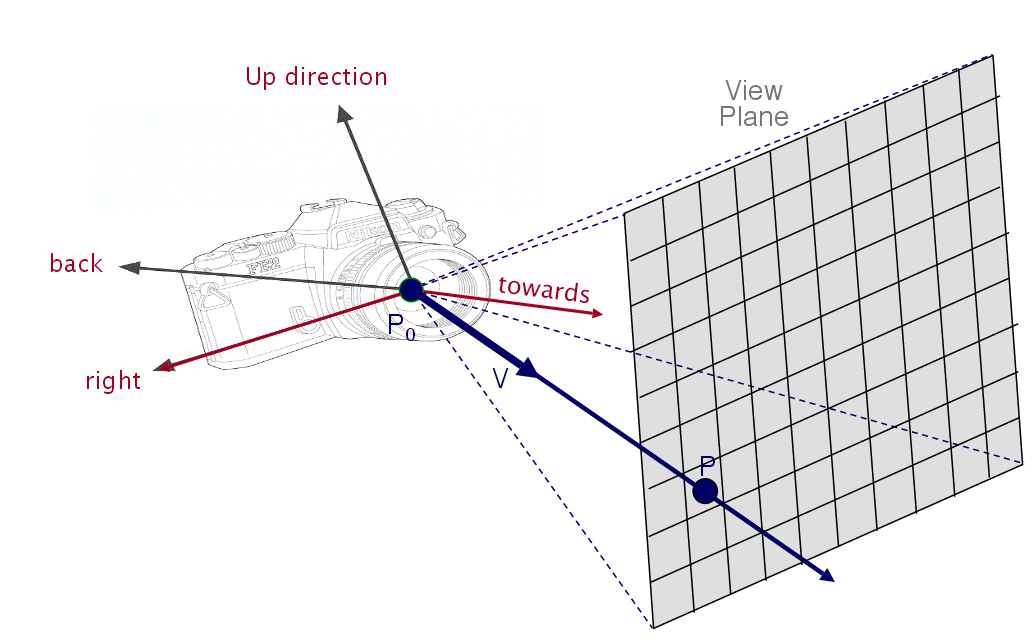
\includegraphics[width=2.5in]{raycast_viewplane}
\caption{Casting a ray through the image plane[5]}
\label{raycast_imageplane}

\end{figure}

\par
Once the ray is defined, the closest triangle (in z) that intersects with the ray is found. This is done in a brute-force approach, iterating through all triangles.
Next, as outlined in the Monte Carlo path tracing algorithm, we recursively reflect the ray up to a set maximum amount of rays (depth), unless the ray hits a light source, in which case the lighting is returned. If no light source is found with the maximum depth, the pixel is deemed to have received no light and is shaded as black.

\begin{figure}[!t]

\centering
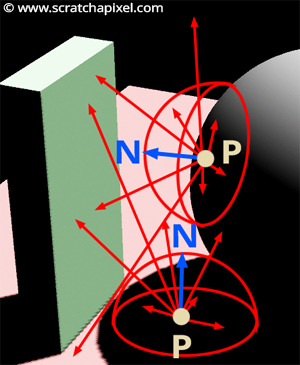
\includegraphics[width=2.5in]{shad2-indirectdiffusehemi.png}
\caption{Random uniform creation of rays in the hemisphere of the collision[6]}
\label{hemisphere rays}

\end{figure}

\begin{figure}[!t]

\centering
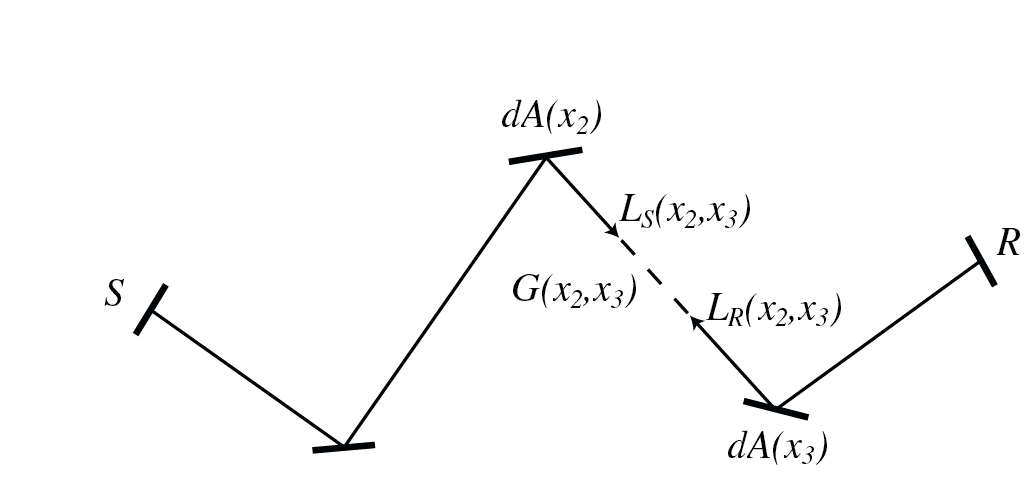
\includegraphics[width=2.5in]{recursive_rays}
\caption{Recursively casting rays between surfaces from the camera to a light source[5]}
\label{recursive_rays}

\end{figure}

\par
For each pixel for which the above process is carried out, it is repeated a certain number of times (or samples), so as to obtain an average which converges to the expected value of lighting for that pixel.


\section{Results}

To test our path tracing application, we placed a grey box floating in an environment that is similar to a typical Cornell Box, but with blue and green walls rather than red and green ones. When running the application with different values of $s$ (ray samples from each pixel) and $d$ (recursion depth), we found that the time of execution was linearly related to the amount of samples, which is unsurprising since $s$ controls the number of iterations of a single loop. When increasing $d$ however, the application appears to converge towards a given time. This can be explained by the geometry of the scene having an average number of reflections before hitting a light source. Therefore, beyond this value for d, the application does not take significantly more time to run. Additionally, an increase in $d$ also increases the brightness of the image, since a ray has a higher chance of hitting a light source if it is allowed a greater number of ``bounces'' off surfaces.

\par
The image becomes sharp at around $s=10$ for any value of $d$, and artifacts persist up to $s=40, d=4$ and $s=100,d=1$.

\begin{figure}[!t]

\centering
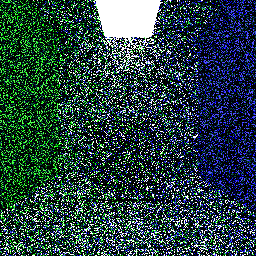
\includegraphics[width=2.5in]{1s_1d_26s}
\caption{1 set of rays, recursion depth 1, time: 26 seconds}
\label{1s_1d_26s}

\end{figure}

\begin{figure}[!t]

\centering
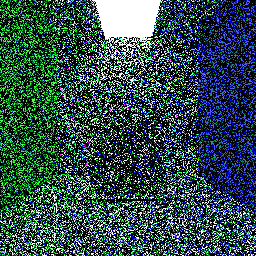
\includegraphics[width=2.5in]{1s_4d_34s}
\caption{1 set of rays, recursion depth 4, time: 34 seconds}
\label{1s_4d_34s}

\end{figure}

\begin{figure}[!t]

\centering
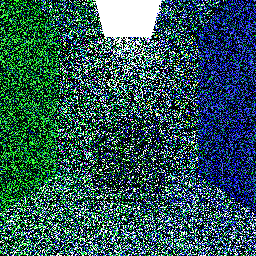
\includegraphics[width=2.5in]{1s_16d_36s}
\caption{1 set of rays, recursion depth 16, time: 36 seconds}
\label{1s_16d_36s}

\end{figure}

\begin{figure}[!t]

\centering
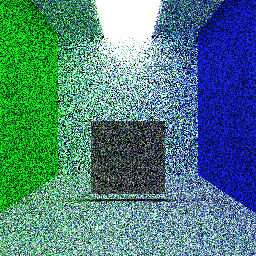
\includegraphics[width=2.5in]{10s_1d_5m42s}
\caption{10 sets of rays, recursion depth 1, time: 5m42s}
\label{10s_1d_5m42s}

\end{figure}

\begin{figure}[!t]

\centering
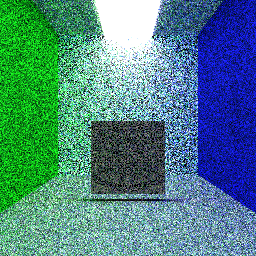
\includegraphics[width=2.6in]{20s_1d_11m26s}
\caption{20 sets of rays, recursion depth 1, time: 11m26s}
\label{20s_1d_11m26s}

\end{figure}

\begin{figure}[!t]

\centering
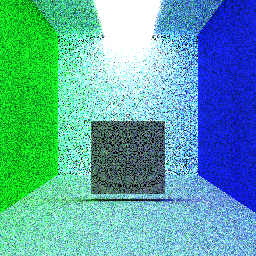
\includegraphics[width=2.5in]{40s_4d_23m25s}
\caption{40 sets of rays, recursion depth 4, time: 23m25s}
\label{40s_4d_23m25s}

\end{figure}

\begin{figure}[!t]

\centering
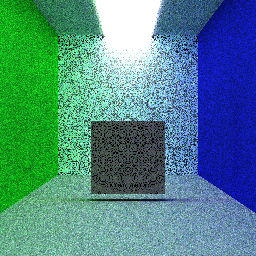
\includegraphics[width=2.5in]{100s_1d_40m21s}
\caption{100 sets of rays, recursion depth 1, time: 40m21s}
\label{100s_1d_40m21s}

\end{figure}

\begin{figure}[!t]

\centering
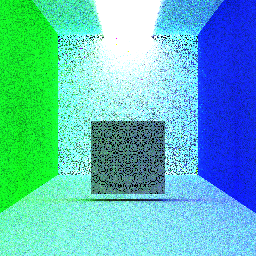
\includegraphics[width=2.6in]{100s_16d_42m10s}
\caption{100 sets of rays, recursion depth 1, time: 42m10s}
\label{1100s_16d_42m10s}

\end{figure}

\section{Challenges \& Observations}
There were many obstacles on the way to the completion of the project. Firstly, the codebase of the assignments is not particularly suited for ray casting: rather, it is suited for processing the geometry one triangle at a time since it rasterized them. Thus, a new architectured had to be written to replace the old one, which was more of a time sink than first anticipated. 
\par
Second, building the scene was a long and tedious process, as the geometry had to be written in the ASCII format as read by the assignment renderer. Exacerbating this process is that path tracing is an expensive algorithm: to test the placement of geometry, the addition of features in the application or to debug it, one must wait between half a minute up to an hour depending on the quality of the generated image.
\par
Additionally, until a late phase of the project, we opted to continue to use the teapot that was featured in all previous assignments. However, since the teapot contains a great number of triangles, it was  expensive to calculate which triangle intersecting with the ray was the closest, since it required iterating through all the triangles. Since this operation was conducted per ray cast, the run-time cost of rendering the teapot was very high.

\section{Further Work}
Because of the limited scope of the project, many features that could be implemented using Monte Carlo path tracing are missing. For example, there is currently no difference between a highly specular and highly diffuse surface because of the uniform random distribution of all reflected rays. Moreover, transparent surfaces and refraction are not simulated again due to the nature of the ray reflectance in the application.

\par
Another opportunity for extension of the application is in its performance. There are two main avanues for this: improvement of runtime complexity and parallelization. In terms of runtime complexity, for determining the closest triangle intersected, one could make use of binary space partition trees rather than a brute force approach. Also, bounding volumes could be used to test for intersection with objects with complex geometries, such as the teapot, which would be encapsulated in a much more simple box shape for collision testing.

\par
As for parallelization, the ray casting approach lends itself well to being parallelized since each ray is reflected irrespective of rays casting through the same pixels (the samples), as well as irrespectively of the rays being cast through other pixels. Therefore, each individual ray could be calculated simultaneously. Incidentally, this process lends itself well to GPUs, which specialize in computing large sets of similar data.

\par
Also, as noted in the result sections, where an increase in $d$ increases brightness, the reflection quantity could be controlled by a random value to keep the shading consistent. This approach is called the Russian Roulette approach, wherein each successive reflected ray diminishes the chance of the next collision producing a reflected ray. This is done by comparing a random value between 0 and 1 to the current weight of the ray, which diminishes with each successive reflection.

\par
Furthermore, for images where $s \ge 10$, fully dark pixels are displayed in a noticeable, somewhat circular pattern. This could be the result of the uniform random reflectance along the semi-circular hemisphere, although there is currently not a definitive answer to why these artifacts appear.

%===================================================

\begin{thebibliography}{5}

\bibitem{Appel}
Appel, A. Some techniques for shading machine renderings of solids. \emph{AFIPS '68 (Spring) Proceedings of the April 30--May 2, 1968, spring joint computer conference}:37-45, 1968.

\bibitem {Whitted}
Whitted, T. An improved illumination model for shaded display. \emph{Comunications of the AMC}, 23(6):343-349, 1980.

\bibitem {Kajiya}
Kajiya, J. The Rendering Equation. \emph{SIGGRAPH '86}, 20(4):143-150, 1986.

\bibitem {Brown}
Slides from Brown University.
\url{http://cs.brown.edu/courses/cs224/papers/mc_pathtracing.pdf}

\bibitem {Virginia}
Slides from the University of Virginia.
\url{http://www.cs.virginia.edu/~gfx/Courses/2010/IntroGraphics/Lectures/6-RayCasting.pdf}

\bibitem {Scratchapixel}
Global Illumination and Path Tracing.
\url{http://www.scratchapixel.com/lessons/3d-basic-rendering/global-illumination-path-tracing/global-illumination-path-tracing-practical-implementation}

\end{thebibliography}

%===================================================

\end{document}
